\graphicspath{{chapters/images/0206/}}

\chapter{Discriminant analysis} 

  In a classification setting, the $Y$ response variable is a categorical
  variable that can indicate to any class $j$ of the $k$ possible classes. The
  aim of classification is estimating the probability of an observation
  $\vec{x}$ belonging to any class $j$, namely 
  
  $$P(Y=j|\vec{X}=\vec{x}),\; j = 1, \dots, k$$ 
  
  Importantly, compared to other methods, discriminant analysis methods are
  usually flexible to any nymber of classes ($2, \dots, k$).
  
  Given the observation $\vec{x}$, what is the probability that it belongs to a
  specific class $j$. In discriminant analysis (LDA, QDA, naive Bayes...),
  contrarily to other methods already seen in the classification setting section
  (\ref{sect: classification}) methods, the values of $P(Y | \vec{X} = \vec{x})$
  are not obtained directly. Instead, the focus is on estimating:
  $$f(\vec{x}|Y=j) = f_j(\vec{x})$$ which basically corresponds to the opposite
  conditional probability. With discriminant analysis methods, first you need to
  assume a distribution of $x$, then you estimate the conditional probability
  density mentioned above (probability density of \vec{x} given a certain class
  $j$). To obtain the other probability, you exploit the Bayes theorem:

  \begin{align*}
  \underbrace{P(Y=j|\vec{X}=\vec{x})}_\text{posterior probability}  
    &= \frac{f(\vec{x}|Y=j)P(Y=j)}{f(\vec{x})}
    & \text{ since } P(A|B) = \frac{P(B|A)P(A)}{P(B)} \\
    &= \frac{f(\vec{x}|Y=j)p(Y=j)}{\sum_{i = 1}^k f(\vec{x}|Y = i)P(Y=i)}
    & \text{ since you have a discrete number of classes} \\\\
    &= \frac{f_j(\vec{x})\overbrace{\pi_j}^\text{\textit{a priori} prob.}}{\sum_{i = 1}^k f_i(\vec{x})\underbrace{\pi_i}_\text{\textit{a priori} prob.}}
    & \text{ just rewriting in a clearer manner}\\
  \end{align*}

  According to Bayes classifier, we choose $j$ that maximises
  $P(Y=j|\vec{X}=\vec{x})$, but since the denominator does not depend on $j$, we
  can just consider the numerator; the problem then becomes assigning $\vec{x}$
  to the class $j$ which maximises $f_i(\vec{x})\pi_j$ (see figure \ref{fig:
  Discriminant analysis decision}).

  \begin{figure}[H]
    \caption{Evaluation process of the class of an observation \vec{x},
    considering only two possible classes, take the class which has higher value
    $f_i(\vec{x})\pi_j$.}
    \centering
    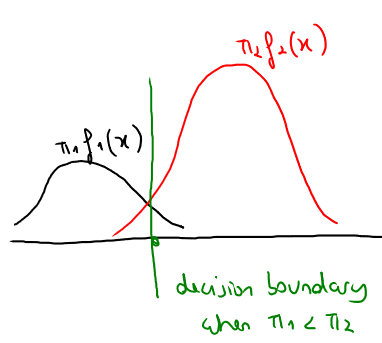
\includegraphics[width=0.45\textwidth]{discAnalysisBoundary}
    \label{fig: Discriminant analysis decision}
    \end{figure}
  

  \section{Estimating the \textit{a priori} probability} In order to estimate
    $\pi_j, \; j=1, \dots, k$, there are two options:
    \begin{itemize}
      \item $\hat{\pi}_j = \nicefrac{1}{k}$, to be used when all $k$ classes are
      equally likely.
      \item $\hat{\pi}_j = \nicefrac{n_j}{n}$ with $n_j$ being the number of
      observations belonging to class $j$ and with $n = n_1 + \dots + n_k$,
      which means assigning to each class a weight dependent on its empirical
      frequence. 
    \end{itemize}

    Instead, $f_j(\vec{x})$ is a p-dimensional density which requires some
    assumptions; the chosen assumptions define which method is used, LDA, QDA or
    naive Bayes. 
  
  \section{Discriminant analysis methods}
    

  \section{Linear discriminant analysis}

    \subsection{LDA with one predictor variable}
      LDA (assuming $p=1$ to make it simple) makes two assumptions:
      \begin{itemize}
        \item \textbf{Gaussianity}, meaning that all classes are gaussian,
        hence:

        $$f_j(x) = \frac{1}{\sqrt{2\pi\sigma^2_j}}
        e^{-\frac{1}{2}\left(\frac{x-\mu_i}{\sigma_j}\right)^2},\;x\in\mathbb{R}$$

        Where:
        \begin{itemize}
          \item $\mu_j$ is the mean
          \item $\sigma_j^2$ is the variance of $X$ conditional on $Y=j$
        \end{itemize}
        
        This assumption does not work if the predictor is discrete.

        \item \textbf{Constant variance}, meaning that different groups, to be
        distinguished by using LDA, have to have \textbf{different means and the
        same variance}:

        $$\sigma_1^2 = \sigma_2^2 = \dots = \sigma_k^2 = \sigma^2$$

      \end{itemize}

      Writing these two assumptions with a single expression we get:
      
      \begin{equation} \label{eq: LDA assumptions}
        (X|Y = j) \sim N(\mu_j, \sigma^2)
      \end{equation}

    \subsection{Linear decision boundary (one predictor)}
      Assume we want to classify an observation $x$ using the LDA method (it is
      correct to use x instead of \vec{x} since in this case we have only a
      single parameter) Starting from the Bayes formula we have:
        \begin{align*}
        P(Y=j|\vec{X}=\vec{x})  
          &= \frac{f_j(\vec{x})\pi_j}{\sum_{i = 1}^k f_i(\vec{x})\pi_i}
          & \text{ rearranged for discriminant analysis}\\
          &= \frac
          {\frac{1}{\sqrt{2\pi\sigma^2}} e^{-\frac{1}{2}\left(\frac{x-\mu_j}{\sigma}\right)^2}\pi_j}
          {\sum_{i = 1}^k\frac{1}{\sqrt{2\pi\sigma^2}} e^{-\frac{1}{2}\left(\frac{x-\mu_i}{\sigma}\right)^2}\pi_i}
          & \text{ because of the assumptions written in formula \ref{eq: LDA assumptions}}\\
          &= \frac
          {e^{-\frac{1}{2}\left(\frac{x-\mu_j}{\sigma}\right)^2}\pi_j}
          {\sum_{i = 1}^k e^{-\frac{1}{2}\left(\frac{x-\mu_i}{\sigma}\right)^2}\pi_i}
          & \text{ simplifying}
        \end{align*}

      We then assign $x$ to the class $j$ which maximises this function, but
      since the denominator does not depend on $j$, it corresponds to maximising
      the numerator, namely
      $$e^{-\frac{1}{2}\left(\frac{x-\mu_i}{\sigma}\right)^2}\pi_j$$ or
      equivalently the logarithm of it
      $$
      \log(\pi_j)-\frac{1}{2}\left(\frac{x-\mu_i}{\sigma}\right)^2 =
      \log(\pi_j)-\frac{x^2}{2\sigma^2} + \frac{x\mu_j}{\sigma}-\frac{\mu_j^2}{2\sigma^2}
      $$
      But since $-\frac{x^2}{2\sigma^2}$ does not depend on $j$ (and because of
      that we consider it as a constant) we can simplify to
      
      \begin{equation*}
        \underbrace{\log(\pi_j) - \frac{\mu_j^2}{2\sigma^2}}_\text{intercept} + x \overbrace{\frac{\mu_j}{\sigma}}^\text{first coefficient $\beta_1$}
      \end{equation*}

      We thus assign $x$ to class $j$ that maximises
      $$\delta_j(x) = \left(\log(\pi_j) -\frac{\mu_j^2}{2\sigma^2}\right) + x
      \left(\frac{\mu_j}{\sigma}\right)$$ and if we define:
      \begin{align*}
      &(\beta_0)_j = \left(\log(\pi_j) -\frac{\mu_j^2}{2\sigma^2}\right) \\
      &(\beta_1)_j = \left(\frac{\mu_j}{\sigma}\right)
      \end{align*}
      We notice that the expression is in linear form:
      $$\delta_j(x) = (\beta_0)_j + x(\beta_1)_j$$ In the case of two classes,
      the \textit{decision boundary} is given by:
      $$\delta_1(x)=\delta_2(x)$$ Which is linear.

    \subsection{Estimating parameters (one predictor)}
      The parameters to use in the LDA method (namely $\pi_1, \dots, \pi_k$,
      $\mu_1, \dots, \mu_k$ and $\sigma^2$) must be estimated. The estimators
      for these parameters are:
      \begin{align*}
      &\hat{\pi}_j = \frac{n_j}{n}
      & \text{ empirical frequency of class }j\\
      &\hat{\mu}_j = \sum_{i:y=j} \frac{x_i}{n_j}
      & \text{ sample mean of class }j\\
      &\hat{\sigma^2} = \frac{\sum_{j=1}^{k}(n_j-1)S_j^2}{\sum_{j=1}^{k}(n_j-1)} = \frac{\sum_{j=1}^{k}\sum_{i:y=j}(x_i-\hat{\mu}_j)^2}{n-k}
      & \text{ pooled variance, $S_j$ is the sample variance}\\
      \end{align*}

      The method assumes homoskedasticity; for this reason, rather than using
      the empirical variance of the individual group, a weighted average of the
      variances of all groups is used. This measure in called pooled variance. 

      Having defined these estimators, $x$ is classified plugging into the
      following equation the values of the estimate  
      $$\hat{\delta_j(x)} = \log(\hat{\pi}_j)
      -\frac{\hat{\mu}_j^2}{2\hat{\sigma^2}} +
      x\frac{\hat{\mu}_j}{\hat{\sigma}}, \; j = 1, \dots, k$$ The class assigned
      is the one producing the highest value of $\delta(x)$.

      
    \subsection{Multivariate LDA}
      We talk about multivariate LDA when $p \geq 1$, meaning that you do not
      have a single predictor variable, as in the example written above, but
      rather a vector of predictors $\vec{X} = (X_1, \dots, X_p)$. In this
      model, the probability of an observation belonging to a certain class $j$
      is \textbf{multivariate normal} distributed, meaning
      $$(\vec{X}|Y=j) \sim N_p(\vec{\mu_j}, \Sigma)$$ Where:
      
      \begin{figure}[h]
        \caption{Multivariate normal distribution. It is shown the case with
        only two variables}
        \centering
        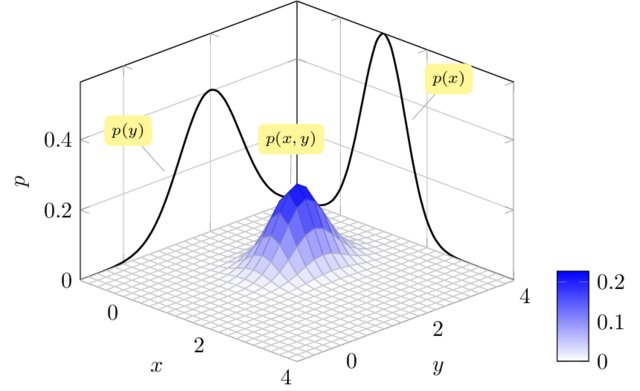
\includegraphics[width=0.7\textwidth]{MultivariateNormalDist}
        \label{fig: Multivariate Normal Distribution}
        \end{figure}
      \begin{figure}[h]
        \caption{Multivariate normal distribution without correlation / with correlation}
        \centering
        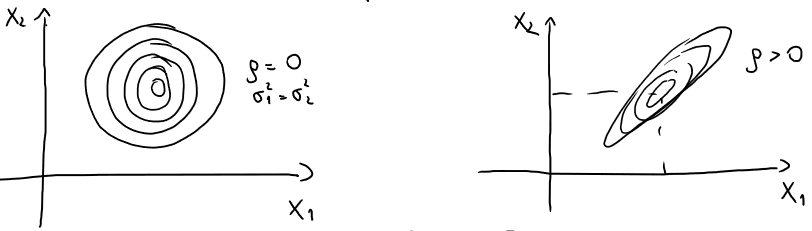
\includegraphics[width=0.7\textwidth]{MultivariateNormalDist-Correlation}
        \label{fig: Multivariate Normal Distribution - Correlation}
        \end{figure}


      \begin{itemize}
        \item $p$ is the number of predictors
        \item $\vec{\mu_j} =
        \begin{pmatrix}\mu_{1j}\\\vdots\\\mu_{pj}\end{pmatrix}$ is a vector of
        mean values (which is class dependent)
        \item $\Sigma = 
          \begin{pmatrix}
            \sigma^2_1   & \sigma_{1,2} & \cdots & \sigma_{1,p}\\
            \sigma_{2,1} & \ddots       &        & \vdots      \\
            \vdots       &              & \ddots & \vdots      \\
            \sigma_{p,1} & \cdots       & \cdots & \sigma_p^{2}\\
          \end{pmatrix}$\\ 
          is the covariance matrix. This model assumes that each of the
          predictors is normal distributed and that the covariance matrix is the
          same for all groups (meaning
          $\Sigma_1=\Sigma_2=\dots=\Sigma_k=\Sigma$). \end{itemize}
          \vspace{\baselineskip}

      Remember that:
      \begin{itemize}
        \item $\sigma_{i,e}=Cov(X_i,X_e)$
        \item $\sigma_{e}^2=Cov(X_e,X_e)=Var(X_e)$
      \end{itemize}
      
    \subsection{Linear decision boundary (multiple predictors)}
      The fact that the decision boundary for LDA is linear can be demonstrated.
      \begin{align*}
      P(Y=j|\vec{X} = \vec{x})
      & = \frac{\pi_jf_j(\vec{x})}{\sum_{i=1}^{k}\pi_if_i(\vec{x})} 
      & \text{ from Bayes formula} \\
      & = \frac
      {\pi_j\frac{1}{(2\pi)^{\nicefrac{p}{2}}|\Sigma|^{\nicefrac{1}{2}}}\exp\left\{-\frac{1}{2}(\vec{x}-\vec{\mu_j})^t \Sigma^{-1} (\vec{x}-\vec{\mu_j})\right\}}
      {\sum_{i=1}^{k}\pi_i\frac{1}{(2\pi)^{\nicefrac{p}{2}}|\Sigma|^{\nicefrac{1}{2}}}\exp\left\{-\frac{1}{2}(\vec{x}-\vec{\mu_j})^t \Sigma^{-1} (\vec{x}-\vec{\mu_j})\right\}}
      & f_j(\vec{x})\sim\text{ multiv. normal}\\
      & = \frac
      {\pi_j\exp\left\{-\frac{1}{2}(\vec{x}-\vec{\mu_j})^t \Sigma^{-1} (\vec{x}-\vec{\mu_j})\right\}}
      {\sum_{i=1}^{k}\pi_i\exp\left\{-\frac{1}{2}(\vec{x}-\vec{\mu_j})^t \Sigma^{-1} (\vec{x}-\vec{\mu_j})\right\}}
      & \text{ simplifying}
      \end{align*}
      We then assign observation $\vec{x}$ to class $j$ which maximises the
      logarithm of the numerator (since the denominator does not depend on $j$)
      \begin{align*}
      \delta_j(\vec{x})
      & = \log(\pi_j) -\frac{1}{2}(\vec{x}-\vec{\mu_j})^t \Sigma^{-1} (\vec{x}-\vec{\mu_j})
      & \text{ function to maximise} \\
      & = \log(\pi_j) -\frac{1}{2}\vec{x}^t\Sigma^{-1}\vec{x} + \vec{x}^t \Sigma^{-1}\vec{\mu_j} - \frac{1}{2}\vec{\mu_j}^t\Sigma^{-1}\vec{\mu_j}
      & \text{ multiplying} \\
      & \propto \left(\log(\pi_j) - \frac{1}{2}\vec{\mu_j}^t\Sigma^{-1}\vec{\mu_j}\right) + \vec{x}^t \left(\Sigma^{-1}\vec{\mu_j}\right)
      & \text{ ignoring terms not depending on } j\\
      & \propto (\beta_0)_j + \vec{x}^t (\vec{\beta})_j
      & \text{ with } (\vec{\beta})_j = (\beta_{1j} \;\cdots\; \beta_{pj})^t \\
      & = \beta_{0j} + x_i\beta_{1j} + x_2\beta_{2j} + \dots + x_p\beta_{pj}
      & \text{ which is linear}
      \end{align*}
      
    \subsection{Estimating parameters (multiple predictors)}
      The estimated parameters are analogous to the single predictor case:
      \begin{align*}
      &\hat{\pi}_j = \frac{n_j}{n}
      & \text{ empirical frequency of class } j\\
      & \vec{\hat{\mu}_j}=\frac{1}{n}\sum_{i:y=j}\vec{x_i}
      & \text{ vector of sample means in class } j\\
      &\hat{\Sigma} = \frac{1}{n-k} \sum_{j=1}^{k}\sum_{i:y=j}(\vec{x_i}-\vec{\hat{\mu}_j})(\vec{x_i}-\vec{\hat{\mu}_j})^t
      & \text{ pooled covariance matrix}\\
      \end{align*}
      
      The class probabilities are obtained when these estimates go into
      $\delta_j(\vec{x})$ leading to
      $$\hat{P(Y=j|\vec{X}=\vec{x})} =
      \frac{e^{\hat{\delta_j}(\vec{x})}}{\sum_{i=1}^{k}e^{\hat{\delta_i}(\vec{x})}}$$
      Since before we used the logarithm function to define $\hat{\delta_j}$, as
      written below:
      $$\hat{\delta_j}(\vec{x}) = \log(\hat{\pi}_j) -
      \frac{1}{2}\vec{\hat{\mu}_j}^t\hat{\Sigma}^{-1}\vec{\hat{\mu}_j} +
      \vec{x}^t \Sigma^{-1}\vec{\hat{\mu}_j}$$

    \subsection{LDA vs logistic regression}
      Assume you want to compare LDA and logistic regression. Take $k=2$ (two possible classes); you
      can then write the log-odds as:
      \begin{align*}
      \text{log-odds}_{LR}
      &= \log\left(\frac{p(1|x)}{1-p(1|x)}\right)
      &= \log\left(\frac{p(1|x)}{p(0|x)}\right)
      &= \delta_1(x)-\delta_0(x)
      &= \beta_0+\beta_1x\\
      \text{log-odds}_{LDA}
      &= \log\left(\frac{p(1|x)}{1-p(1|x)}\right)
      &= \log\left(\frac{p(1|x)}{p(0|x)}\right)
      &= \delta_1(x)-\delta_0(x)
      &= \alpha_0+\alpha_1x
      \end{align*}

      Both of them generate linear expressions
      
      % #TODO this is not the correct term

      The main difference, assuming that $f_i(\vec{x})$ can be approximated by a
      multivariate normal, is the estimation of parameters:
      \begin{itemize}
        \item LR: $\vec{\hat{\beta}}$ is estimated directly by Maximum
        Likelihood 
        \item LDA: $\vec{\hat{\alpha}}$ are estimated indirectly via
        $\vec{\hat{\mu_j}}$, $\hat{\Sigma}$
      \end{itemize}
      Logistic regression optimization procedure is more unstable when the
      classes are well separated (probability close to $0$ and $1$).

  \section{Quadratic discriminant analysis}
    Quadratic discriminant analysis (QDA) is similar to LDA in the sense that it
    is still defined as a multinormal distribution, but the assumption of
    homoskedasticity falls; this means that you assume all predictor variables
    to be normal distributed but each of them can have its own covariance
    matrix. Importantly, QDA assumes still gaussianity. Therefore we can write
    QDA as
    $$(\vec{X}|Y=j) \sim N_p(\vec{\mu_j}, \Sigma_j)$$

    \subsection{Quadratic boundary}
      For QDA it can be shown that the decision boundary is quadratic. The
      calculations shown below prove it

      \begin{align*}
      P(Y=j|\vec{X} = \vec{x})
      & = \frac{\pi_jf_j(\vec{x})}{\sum_{i=1}^{k}\pi_if_i(\vec{x})} 
      & \text{ from Bayes formula} \\
      & = \frac
      {\pi_j\frac{1}{(2\pi)^{\nicefrac{p}{2}}|\Sigma_j|^{\nicefrac{1}{2}}}\exp\left\{-\frac{1}{2}(\vec{x}-\vec{\mu_j})^t \Sigma^{-1}_j (\vec{x}-\vec{\mu_j})\right\}}
      {\sum_{i=1}^{k}\pi_i\frac{1}{(2\pi)^{\nicefrac{p}{2}}|\Sigma_i|^{\nicefrac{1}{2}}}\exp\left\{-\frac{1}{2}(\vec{x}-\vec{\mu_j})^t \Sigma^{-1}_i (\vec{x}-\vec{\mu_j})\right\}}
      & \text{ from the assumptions} \\
      & = \frac
      {\pi_j|\Sigma_j|^{-\nicefrac{1}{2}}\exp\left\{-\frac{1}{2}(\vec{x}-\vec{\mu_j})^t \Sigma^{-1}_j (\vec{x}-\vec{\mu_j})\right\}}
      {\sum_{i=1}^{k}\pi_i|\Sigma_i|^{-\nicefrac{1}{2}}\exp\left\{-\frac{1}{2}(\vec{x}-\vec{\mu_j})^t \Sigma^{-1}_i (\vec{x}-\vec{\mu_j}\right)\}}
      & \text{ simplifying}
      \end{align*}

      Then assign observation $\vec{x}$ to class $j$ which maximises the
      logarithm of the numerator (since the denominator does not depend on $j$).
      \begin{align*}
      \delta_i(\vec{x}) 
      & = \log(\pi_j) -\frac{1}{2}\log(|\Sigma_j|) -\frac{1}{2}(\vec{x}-\vec{\mu_j})^t \Sigma^{-1}_j (\vec{x}-\vec{\mu_j}) 
      & \text{ function to maximise}\\
      & = \log(\pi_j) -\frac{1}{2}\log(|\Sigma_j|) -\frac{1}{2}\vec{x}^t\Sigma^{-1}_j\vec{x} + \vec{x}^t \Sigma^{-1}_j\vec{\mu_j} - \frac{1}{2}\vec{\mu_j}^t\Sigma^{-1}_j\vec{\mu_j}
      & \text{ multiplying}\\
      & =\overbrace{-\frac{1}{2}\vec{x}^t\Sigma^{-1}_j\vec{x}}^\text{quadratic term} + \overbrace{\vec{x}^t \Sigma^{-1}_j\vec{\mu_j}}^\text{linear term} + \overbrace{\log(\pi_j) -\frac{1}{2}\log(|\Sigma_j|)}^\text{intercept}
      & \text{ which is quadratic in } \vec{x}\\
      \end{align*}

    \subsection{LDA vs QDA}

      \begin{figure}[H]
        \caption{QDA vs LDA}
        \centering
        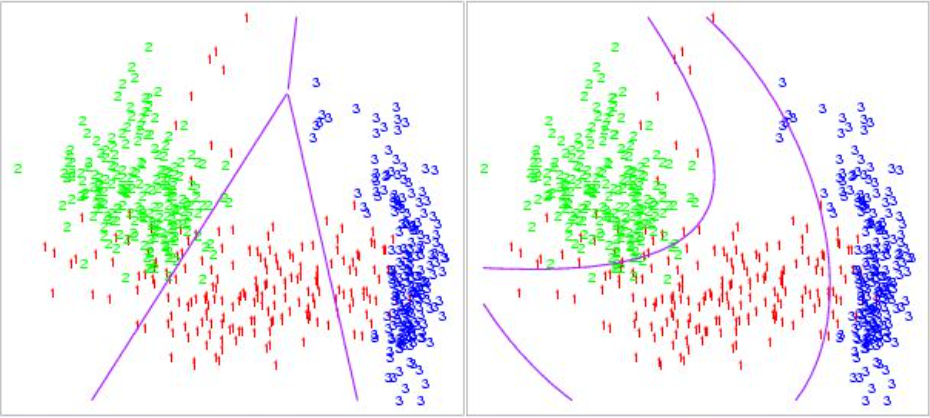
\includegraphics[width=0.7\textwidth]{QDAvsLDA}
        \label{fig: QDA vs LDA}
        \end{figure}
    


      Obviously, lines generated through QDA are always curved, contrarily to
      LDA; then, they are more prone to overfit the data. QDA has more
      parameters than LDA, in fact in the first case the number of parameters is kxp parameters
      
      % #TODO write clearer this part
      
      namely
      \begin{align*}
        \text{QDA: } & pk + k\frac{p(p+1)}{2} 
        &\vec{\mu_1},\dots,\vec{\mu_k},&\;\Sigma_1,\dots,\Sigma_k\\
        \text{LDA: } & pk + \frac{p(p+1)}{2}
        &\vec{\mu_1},\dots,\vec{\mu_k},&\;\Sigma_{p\times p}
      \end{align*}

      For example, if we take $k=2$ and $p=50$, then LDA has 1375 parameters,
      while QDA has 2650. Because of the greater amount of parameters, the variability/balance equilibrium has to be evaluated. In case of equivalent results, it is important to take the simpler model.
